\documentclass[a4paper]{scrreprt}
 
\usepackage[german]{babel}
\usepackage[utf8]{inputenc}
\usepackage[T1]{fontenc}
\usepackage{ae}
\usepackage[bookmarks,bookmarksnumbered]{hyperref}
\usepackage{graphicx}
\usepackage{floatflt}
\usepackage{enumitem}
\usepackage{pifont}
\setlength{\parindent}{0pt}
 
\begin{document}
 
\title{Pflichtenheft}
\subtitle{ILIAS Review Plugin}
\publishers{Version: 5.0, Status: Fertiggestellt}
\author{SWT-Gruppe 04\\ \\Auftraggeber: Thordis Kombrink\\Weitere: Dr Birgit Demuth, Professor Wollersheim\\Tutor: Andy Püschel}
\maketitle

\begin{abstract}
\Huge{Zusammenfassung}\\\normalsize
Dieses Pflichtenheft wurde von der Gruppe 4 des Softwaretechnologie-Projekts, 2014/15 entwickelt. Es beschreibt konkret, wie das Team die Anforderungen der Kundin Thordis Kombrink und der Stakeholder Dr. Birgit Demuth und Professor Wollersheim zu lösen gedenkt. Erst wenn der Auftraggeber das Pflichtenheft akzeptiert, sollte die eigentliche Arbeit im Team beginnen.
\vspace{1cm}
 
\huge{Historie}\\\normalsize
\begin{tabular}[c]{|l|l|l|l|l|}\hline
Version & Status & Datum & Autor(en) & Erläuterung\\\hline
1.0 & In Arbeit & 29.10.14 & Team Ilias & Grundlegender Aufbau des Pflichtenhefts\\\hline
2.0 & In Arbeit & 4.11.14 & Team Ilias & Formatierung und Komplettierung des PH \\\hline
3.0 & In Arbeit & 8.11.14 & Team Ilias & Überarbeitung-Diagramme und Anforderung \\\hline
4.0 & In Arbeit & 11.11.14 & Team Ilias & Anwendungsfallbeschreibung\\\hline
5.0 & fertiggestellt & 12.11.14 & Team Ilias & Abschließen der Diagramme und GUI\\\hline
\end{tabular}
\vspace{0.5cm}
 
\huge{Reviewnachweis}\\\normalsize
\begin{tabular}[c]{|l|l|l|l|l|}\hline
Version & Status & Datum & Autor(en) & Erläuterung\\\hline
2.0 & In Arbeit & 5.11.14 & Team Ilias & Überprüfung des Pflichtenhefts, Überarbeitung\\
&&&& der Diagramme und Anforderungen\\\hline
4.0 & In Arbeit & 11.11.14 & Team Ilias & Besprechung der GUI und Ablaufproezess eines\\
&&&& Review-Durchgangs\\\hline
\end{tabular}
\end{abstract}


% Platzierung des Inhaltsverzeichnisses
\tableofcontents
 
\chapter{Aufgabenstellung und Zielsetzung}
Aufgabe ist es ein Plugin für das freie, internetbasierte Lernsystem ILIAS\footnote{\url{http://www.ilias.de/docu/ilias.php?baseClass=ilrepositorygui&reloadpublic=1&cmd=frameset&ref_id=1}} zu programmieren, um es um eine Review-Möglichkeit der erstellten Fragen zu erweitern. 
 
\section{Qualitätsziele}
\begin{tabular}{|c|c|c|c|c|}\hline
Anforderung & Sehr wichtig & Wichtig & Normal & Irrelevant \\\hline
Funktionalität &\ding{51}&&&\\\hline
Benutzerfreundlichkeit &\ding{51}&&&\\\hline
Erweiterbarkeit &&\ding{51}&&\\\hline
Zuverlässigkeit &&\ding{51}&&\\\hline
Korrektheit &&\ding{51}&&\\\hline
Sicherheit &&&\ding{51}&\\\hline	
Effizienz &&&\ding{51}&\\\hline
Portierbarkeit &&&&\ding{51}\\\hline

\end{tabular}

         
\chapter{Fachlicher Überblick}
ILIAS, kurz für Integriertes Lern-, Informations- und Arbeitskooperations-System, ist eine freie E-Learning Online-Anwendung. In dieser gibt es Lehrkräfte und Studenten. Lehrkräfte können Fragen erstellen, die in Fragenpools gesammelt werden. Aus diesen Fragepools können durch die Lehrkräfte Fragen für einen Test ausgewählt werden, der anschließend von Studenten beantwortet werden soll. \\
Um die Qualität der verwendeten Fragen zu gewährleisten, soll ein Review-System entwickelt werden, durch welches Lehrkräfte erstellte Fragen anderer Lehrkräfte überprüfen und bewerten können.\\
Dadurch entsteht ein aktiver Fragen-Enwicklungsprozess.\\

\chapter{Anforderungen}

 
\section{Musskriterien}
Das Plugin muss die ILIAS-Version 4.4.5, die MySQL Version 5.0.11 und die PHP-Version 5.5.11 unterstützen.\\
Das Plugin soll bevorzugt an Lehrstühlen zur Verfügung stehen.

Die fachlichen Anforderungen sind:
\begin{enumerate}[label= FA \arabic*:]
\item Es soll ein Plugin zur Implementierung von reviewbaren Fragen erstellt werden.
\item Eine reviewbare Frage soll alle Eigenschaften einer normalen Ilias-Frage besitzen.
\item Es soll ein Plugin zur Verwaltung von reviewbaren Fragen und Reviews geschrieben werden.
\item Es soll eine Übersicht-Benutzeroberfläche zur Verwaltung von reviewbaren Fragen und Reviews geben.
\item Es soll eine Eingabe-Benutzeroberfläche geben, die zur Eingabe der Reviewdaten dient.
\item Die Eingabe-Benutzeroberfläche soll nur Personen bereitstehen, die ausgewählt wurden, um ein Review zu beantworten.
\item Die Eingabe-Benutzeroberfläche soll bereits bestehende Daten eines Reviews anzeigen können.
\item Alle über die Eingabe-Benutzeroberfläche eingegebenen Daten sollen gespeichert werden.
\item Es soll eine Ausgabe-Benutzeroberfläche geben, die zur Ausgabe von Reviews dient.
\item Die Ausgabe-Benutzeroberfläche soll einem Autor, einem Reviewer und einem Administrator bereitstehen.
\item Es soll eine Zuweisungs-Benutzeroberfläche zur Zuweisung von Reviewern zu Autoren geben.
\item Die Zuweisungs-Benutzeroberfläche soll nur Administratoren bereitstehen.
\item Ein Autor soll alle von ihm erstellten reviewbaren Fragen als Übersicht sehen können.
\item Ein Autor soll keine Namen von Personen sehen, die ausgewählt wurden, um Reviews zu seinen Fragen zu erstellen.
\item Ein Autor soll zu einer reviewbaren Frage, zu der noch keine Reviews angefordert wurden, Reviews anfordern können.
\item Ein Autor soll nach Bearbeitung einer reviewbaren Frage zur neuen Version der Frage neue Reviews  anfordern können.
\item Ein Autor soll die zu einer reviewbaren Frage, zu der bereits Reviews angefordert wurden, zugehörigen Reviews in einer Ausgabe-Benutzeroberfläche öffnen können.
\item Ein Reviewer soll alle von ihm beantworteten und noch zu beantwortende Reviews als Übersicht sehen können.
\item Ein Reviewer soll ein von ihm noch nicht beantwortetes Review zur Eingabe in einer Eingabe-Benutzeroberfläche öffnen können.
\item Ein Reviewer soll ein von ihm bereits beantwortetes Review zur Einsicht in einer Ausgabe-Benutzeroberfläche öffnen können.
\item Ein Administrator soll den Namen eines zu einem Review zugehörigen Reviewers sehen können.
\item Ein Administrator soll über eine Zuweisungs-Benutzeroberfläche Autoren Reviewer zuweisen können.
\item Wenn zu einer reviewbaren Frage Reviews angefordert werden, sollen automatisch die dem Autor der reviewbaren Frage zugeordneten Reviewer per Nachricht informiert und aufgefordert werden, dass ihnen zugeordnete Review zu beantworten.
\item Wenn ein Review ausgefüllt wurde, soll der Autor der zum Review zugehörigen Frage per Nachricht informiert werden.
\item Reviews sollen den Reviewern einer Gruppe entweder per Zufall oder manuell über eine Eingabemaske zugeordnet werden.
\item Der Nutzer soll stets dazu aufgefordert werden  vor dem Absenden des Formulars  leere Formularfelder auszufüllen.  
\item Fragen sollen manuell vom Gruppenadministrator freigegeben werden können, um das Reviewing auch außerhalb von Ilias zu ermöglichen.
\end{enumerate}


Die nicht-fachlichen Anforderungen sind:
\begin{enumerate}[label=NFA \arabic*:]
\item Es soll Sprachunterstützung für Deutsch und Englisch bereitgestellt werden.
\item Das Plugin nutzt die in ILIAS vorhandenen Plugin-Schnittstellen.
\end{enumerate}


\section{Kannkriterien}
Ein Kannkriterium ist die Itemkonstruktion:
\begin{itemize}
\item Der Fragepool kann sortiert werden nach:
\begin{itemize}
\item Thema
\item Themenbereich
\item Learning Outcome
\item Inhalt
\end{itemize}
\item Die Sortierung ist frei wählbar
\end{itemize}
Das zweite Kannkriterium ist der Blueprint:
\begin{itemize}
\item Bei der Erstellung einer Klausur ist auswählbar, wieviele Fragen sie beinhalten soll.
\item Die Fragen werden nach den Kriterien Taxonomiestufe und Themenbereich ausgewählt. 
\item Die Klausur wird dementprechend aus den Fragen erstellt.
\end{itemize}
Ein drittes Kannkriterium ist eine Fragenhistory:
\begin{itemize}
\item Wenn eine Frage bearbeitet wird, soll die alte Version der Frage weiter gespeichert werden.
\item Alle zu einer so gespeicherten Frage zugehörigen Reviews sollen ebenfalls gespeichert werden.
\end{itemize}



\section{Konventionen}
Es gelten die im 'Ilias-Developement-Guide'\footnote{\url{http://www.ilias.de/docu/goto.php?target=lm_42&client_id=docu} (29.10.14)} und in den 'Ilias Usability and Accessibility Guidelines'\footnote{\url{http://www.ilias.de/docu/goto_docu_lm_459.html} (29.10.14)} festgesetzten Konventionen.

\chapter{Top-Level-Architektur}
\section{Top-Level-Architektur}
Für die Reviews sind mehrere Plugins notwendig. Zum einen soll ein Plugin entwickelt werden, das die Verwaltung von Reviews ermöglicht, zum anderen müssen Plugins für Reviewbare Fragen erstellt werden. Das Review-Plugin stellt die Benutzeroberflächen bereit und beinhaltet die Review-Datenbank.\\
Als Beispiel für ein Plugin einer reviewbaren Frage wurde das Plugin der reviewbaren Multiple-Choice-Frage gewählt.\\
Für die Plugins werden verschiedene Plugin-Slots verwendet. Ilias stellt eine Schnittstelle für neue Fragen bereit. Das Verwaltungs-Plugin soll als Repository-Plugin erstellt werden.\\ 
(siehe nächste Seite)\\

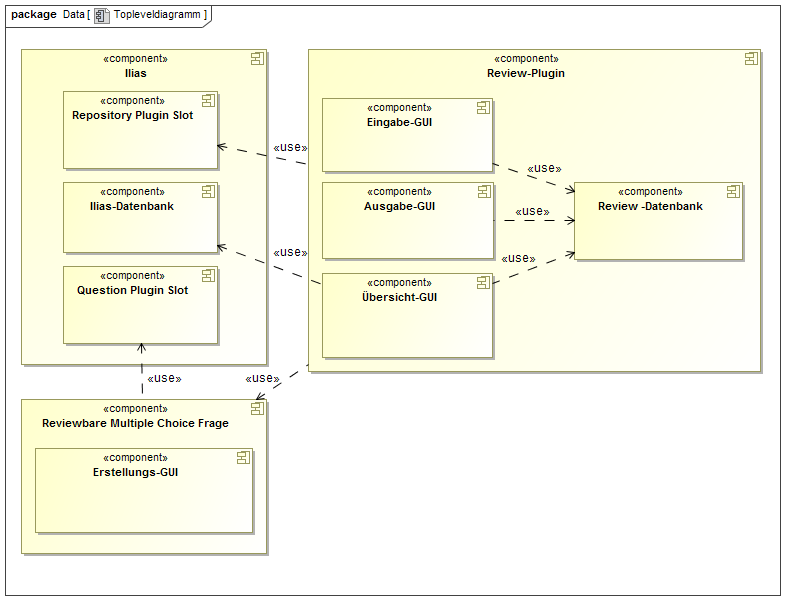
\includegraphics[width=1.0\textwidth]{Component_Diagram__Topleveldiagramm.png}
\label{Toplevel-Architektur}

\chapter{Datenmodell}
\section{Analyseklassendiagramm}
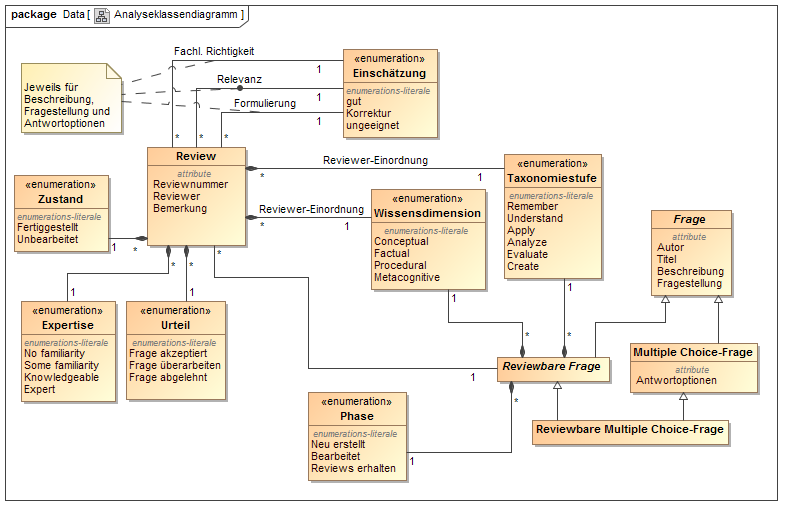
\includegraphics[width=1.0\textwidth]{Class_Diagram__Analyseklassendiagramm.png}
\label{Analyseklassendiagramm}
 
\section{Klassen}
\texttt{Review}\\
Alle Reviews sind intern mit einer Nummerierung versehen und eindeutig einer Frage zugeordnet, wobei zu einer Frage beliebig viele Reviews vorhanden sein können. Ein Review beinhaltet die Einschätzung des Reviewers hinsichtlich der fachlichen Richtigkeit, Relevanz und Formulierung der Beschreibung, Fragestellung und Antwortoptionen einer Frage. Zusätzlich gibt der Reviewer die von ihm bevorzugte Einordnung der Frage in Taxonomiestufe und Wissensdimension an. Außerdem beinhaltet ein Review das Urteil des Reviwers und weitere Bemerkungen, die je nach Urteil Anmerkungen zur Überarbeitung oder eine Begründung der Ablehnung darstellen. Zusätzlich werden der Name des Reviewers, seine selbsteingeschätzte Expertise und der Zustand des Reviews gespeichert.\\
\texttt{Frage}\\
Allen Fragen, die in Ilias erstellt werden können, ist gemein, dass sie über einen Autor, einen Titel, die eigentliche Fragestellung und eine weiterführende Beschreibung verfügen.\\

\texttt{Reviewbare Frage}\\
Um das Review-Plugin zu verwirklichen, muss zu jeder Frage noch ihre Taxonomiestufe und Wissensdimension gespeichert werden. Zusätzlich ist die Angabe der vom Autor gewünschten Anzahl an Reviews erforderlich.\\

\texttt{Multiple Choice-Frage}\\
Eine Multiple Choice-Frage ist ein in Ilias existierender Fragetyp, der über alle Eigenschaften einer Frage und eine beliebige Anzahl an Antwortoptionen verfügt.\\

\texttt{Reviewbare Multiple Choice-Frage}\\
Eine Reviewbare Multiple Choice-Frage ist eine Multiple-Choice Frage, die zusätzlich über die Eigenschaften einer Reviewbaren Frage verfügt und steht exemplarisch für einen Fragetyp, der für das Review-Plugin verwendet werden kann.
\section{Enumerationen}
\texttt{Taxonomiestufe}\\
Die Taxonomiestufe wird vom Reviewer angegeben und repräsentiert die Einschätzung der intellektuellen Anforderungen an den Geprüften.\\

\texttt{Wissensdimension}\\
Die Wissensdimension wird vom Reviewer angegeben und beschreibt, auf welchen Wissensbereich der Gefragte zurückgreifen muss.\\

\texttt{Urteil}\\
Das Urteil gibt an, ob der Reviewer die Frage so akzeptiert, meint, dass sie überarbeitet werden muss oder ablehnt.\\

\texttt{Expertise}\\
Mit der Expertise gibt der Reviewer an, wie gut er sich auf dem Fachgebiet der gestellten Frage auskennt.\\

\texttt{Einschätzung}\\
Die Einschätzung des Reviewers sagt für jeden Punkt aus, ob er gut ist, einer Korrektur bedarf oder für ungeeignet befunden wurde.\\

\texttt{Zustand}\\
Ein Review gilt nach der Einladung des Reviewers durch den Autor so lange als unbearbeitet, bis der Reviewer es durch Bearbeitung fertiggestellt hat.
\chapter{Anwendungsfälle}
Das Review Plugin deckt zwei Anwendungsfälle ab: 

\section{Anwendungsfalldiagramm}
\texttt{Review}\\

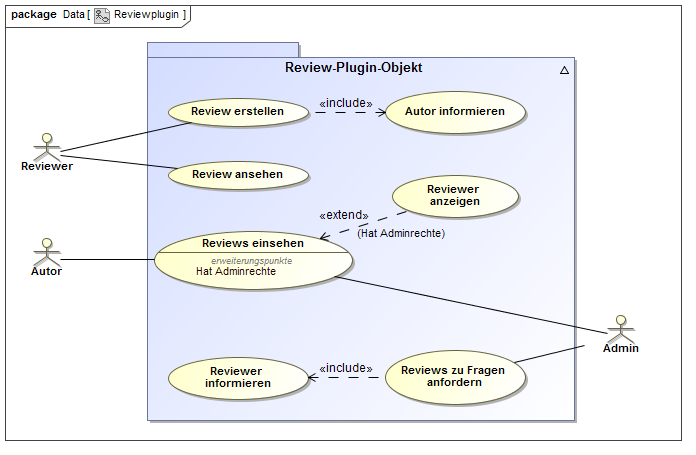
\includegraphics[width=1.0\textwidth]{Use_Case_Diagram__Reviewplugin.png}
\label{Review}

\begin{tabular}{|p{0.5cm}|p{3cm}|p{0.5cm}|p{4cm}|p{4.5cm}|}\hline
Nr. & Anwendungsfall & Nr. & Anfrage & Antwort\\\hline
1.0 & Ein Autor fordert Reviews & 1.1 & Es ist noch kein Review vorhanden & Es werden neue Reviewer ausgewählt und ihnen zugeordnete, unbearbeitete Reviews erstellt. Die Reviewer werden darüber informiert, dass sie ein Review zu schreiben haben.\\\hline
&&1.2 & Es sind bereits Reviews zu der Frage vorhanden. & Die bereits vorhandenen Reviews werden auf unbearbeitet gesetzt. Die Reviewer werden darüber informiert.\\\hline
2.0 & Reviewer erstellt ein Review & 2.1 & Der Reviewer füllt alle Felder vollständig aus. & Das Review wird auf bearbeitet gesetzt und in der Datenbank gespeichert. Zudem wird vermerkt das wievielte Review der Reviewer gegeben hat.\\\hline
&&2.2 & Der Reviewer vergisst, Felder auszufüllen. & Der Reviewer erhält eine Meldung, dass er vergessen hat manche Felder auszufüllen. \\\hline
3.0 & Reviewer betrachtet Reviews & 3.1 & Der Reviewer versucht Reviews einzusehen & Der Reviewer erhält eine Übersicht nur über das von ihm gegebene Review. \\\hline
4.0 & Autor betrachtet Reviews & 4.1 & Es sind Reviews vorhanden & Der Autor erhält eine Übersicht über alle bereits gegebenen Reviews, allerdings kann er die Informationen zu den Reviewern nicht einsehen. \\\hline
5.0 & Administrator betrachtet Reviews & 5.1 & Es sind Reviews vorhanden & Der Administrator erhält eine vollständige Übersicht über die gegebenen Reviews. \\\hline
\end{tabular}
 
\newpage
\texttt{Fragepool}\\

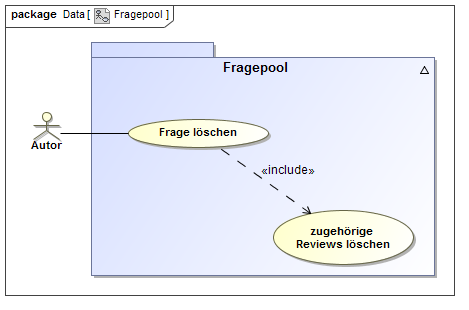
\includegraphics[width=1.0\textwidth]{Use_Case_Diagram__Fragepool.png}
\label{Fragepool bearbeiten}

\begin{tabular}{|p{0.5cm}|p{3cm}|p{0.5cm}|p{4cm}|p{4.5cm}|}\hline
Nr. & Anwendungsfall & Nr. & Anfrage & Antwort\\\hline
1.0 & Autor löscht eine Frage & 1.1 & Reviews vorhanden & Zugehörige Reviews werden gelöscht\\\hline
\end{tabular}

\section{Akteure}
(Hier wird Ilias als eine Lernumgebung für Universitäten behandelt!)\\
Mit Ilias arbeiten Professoren (Arbeitsgruppen-Admin), die in der Lage sind E-Klausuren zu erstellen. Zur Arbeitsgruppe gehören Tutoren (Gruppenmitglieder), die in der Lage sein sollen, die E-Klausuren einzusehen und zu jeder Frage ein Review abzugeben. Die Studenten haben keinen Zugriff in den Entwicklungsprozess der Fragen.

\newpage
\section{Sequenzdiagramme}
\texttt{Review anfordern}\\
Nachdem der Autor eine Frage erstellt hat, kann er ein Review anfordern. Dadurch werden Reviewer bestimmt, welche vom Review-Plugin informiert werden, dass ein Review abzugeben ist.\\

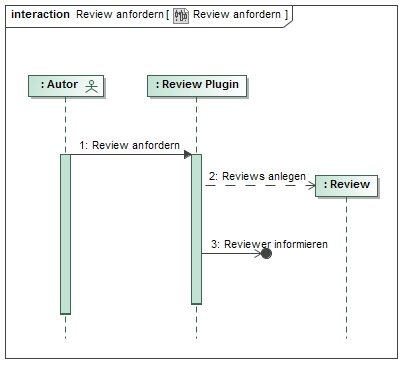
\includegraphics[width=1.0\textwidth]{Sequence_Diagram__Review_anfordern__Review_anfordern.png}
\label{Review anfordern}

\newpage
\texttt{Review abschließen}\\
Wenn ein Reviewer sein Review abgeschlossen hat, werden die Review-Daten formatiert und abgespeichert. Im Anschluss wird der Autor informiert, dass ein neues Review vorhanden ist.\\

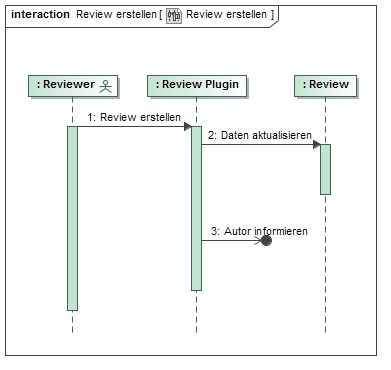
\includegraphics[width=1.0\textwidth]{Sequence_Diagram__Review_erstellen__Review_erstellen.png}
\label{Review beenden}




\chapter{Dialoge(GUI-Prototyp)}
Das Interface für die Revieweingabe wurde bereits von Frau Kombrink vorgegeben und so wie es designtechnisch auch möglich ist wird diese Vorgabe auch umgesetzt.\\
Die Ausgabeoberfläche eines Reviews soll der Eingabeoberfläche entsprechen. Natürlich sollen alle Eingabefelder bereits mit den Werten ausgefüllt und auf 'readonly' gesetzt sein, sodass der Betrachter das Review nicht mehr überarbeiten kann.
(siehe nächste Seite)
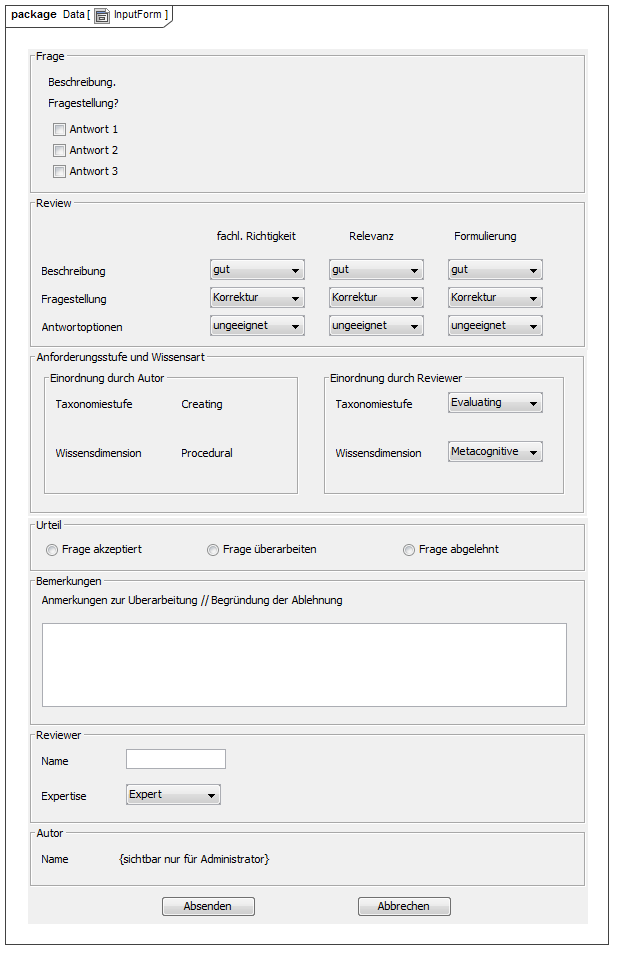
\includegraphics[width=0.99\textwidth]{User_Interface_Modeling_Diagram__InputForm.png}
\label{Grafische Benutzeroberfläche}\\
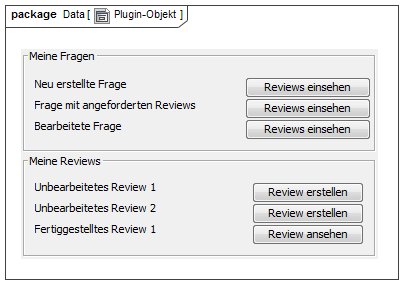
\includegraphics[width=0.99\textwidth]{User_Interface_Modeling_Diagram__Plugin-Objekt.png}
\label{Grafische Benutzeroberfläche Autor}
\\
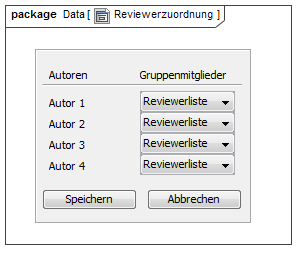
\includegraphics[width=0.7\textwidth]{User_Interface_Modeling_Diagram__Reviewerzuordnung.png}
\label{Grafische Benutzeroberfläche Autor}


\chapter{Akzeptanztestfälle}
Werden funktionale Anforderungen im Gebrauch erfüllt?
Anforderungen werden aus den Anwendungsfall- und Sequenzdiagrammen abgeleitet!
Pro Anwendungsfall ein Sequenzdiagramm (beschreibt Szenario).
Für jedes Szenario sollte es einen Akzeptanztestfall geben.\\

\begin{tabular}{|p{0.5cm}|p{2cm}|p{2.5cm}|p{3cm}|p{2cm}|p{2cm}|}\hline
ID & Testfallbez.&Testobjekte&Ausgangssituation&Eingabewert&Sollresultat \\\hline
1 & Frage löschen &&&&\\\hline
2 & Frage anzeigen &&Es existiert eine Frage&&\\\hline
3 & Review erstellen &&&&\\\hline
4 & Review anzeigen &&Es existiert ein Review&&\\\hline
4.1 & Review anzeigen &&Es existiert kein Review	&&\\\hline
5 & Review anfordern &&Es existiert mindestens ein Review&&\\\hline
5.1 & Review anfordern &&Es existiert kein Review&&\\\hline
\end{tabular}\\
Anmerkung: Akzeptanztestfälle (User Acceptance Test) werden eigentlich vom Kunden vorgenommen.
 
% Abbildungsverzeichnis
%\listoffigures
 
\end{document}